\documentclass[a4paper,11pt, oneside]{report}

\usepackage[utf8] { inputenc }
\usepackage[T1] { fontenc } 
\usepackage[english]{babel}
\usepackage{titlesec, blindtext, color}
\definecolor{gray75}{gray}{0.75}
\newcommand{\hsp}{\hspace{20pt}}

\usepackage{amsmath}
\usepackage{amsthm}
\usepackage{amssymb}
\usepackage[titletoc]{appendix}
\usepackage{array}
\usepackage{booktabs}
\usepackage{float}
\usepackage{braket}
\usepackage{fullpage}
\usepackage{graphicx}
\usepackage{hyperref}
\usepackage{titlepic}
\usepackage [round,authoryear] {natbib}
\usepackage{ifthen}
\newtheorem{axiom}{Axiom}
\newtheorem{theorem}{Theorem}
\newtheorem{definition}{Definition}

\usepackage{algorithm}
\usepackage{algpseudocode}
\usepackage{amsmath}
\usepackage{vhistory}
\usepackage{xcolor}
\usepackage{afterpage}
\usepackage{tikz}
\usepackage{transparent}
\usepackage{geometry}
\usepackage{caption}
\usepackage{subcaption}

% Custom colours
\definecolor{bestseller-grey}{RGB}{216, 216, 215}


% Do not show subsections in table of contents
\setcounter{tocdepth}{1}

% Python code setup
\usepackage{pythonhighlight}

\DeclareMathOperator*{\argmax}{argmax}
\DeclareMathOperator*{\argmin}{argmin}

\theoremstyle{definition}
\newtheorem{exinn}{Example}
\newenvironment{example}
{\clubpenalty=10000
	\begin{exinn}%
		\mbox{}%
		{\color{black}\leaders\hrule height .8ex depth \dimexpr-.8ex+0.8pt\relax\hfill}%
		\mbox{}\linebreak\ignorespaces}
	{\par\kern2ex\hrule\end{exinn}}

% COMMANDS FOR REFERENCES
\newcommand{\chref}[1]{\hyperref[#1]{Chapter~\ref{#1}}}
\newcommand{\secref}[1]{\hyperref[#1]{Section~\ref{#1}}}
\newcommand{\subsecref}[1]{\hyperref[#1]{Subsection~\ref{#1}}}
\newcommand{\tabref}[1]{\hyperref[#1]{Table~\ref{#1}}}
\newcommand{\figref}[1]{\hyperref[#1]{Figure~\ref{#1}}}
\newcommand{\appref}[1]{\hyperref[#1]{Appendix~\ref{#1}}}
\newcommand{\lstref}[1]{\hyperref[#1]{Listing~\ref{#1}}}
\newcommand{\EQref}[1]{\hyperref[#1]{Equation~\ref{#1}}}
\newcommand{\dfref}[1]{\hyperref[#1]{Definition~\ref{#1}}}
\renewcommand{\algref}[1]{\hyperref[#1]{Algorithm~\ref{#1}}}

\newcommand{\chrefpage}[1]{\hyperref[#1]{Chapter~\vref{#1}}}
\newcommand{\secrefpage}[1]{\hyperref[#1]{Section~\vref{#1}}}
\newcommand{\subsecrefpage}[1]{\hyperref[#1]{Subsection~\vref{#1}}}
\newcommand{\tabrefpage}[1]{\hyperref[#1]{Table~\vref{#1}}}
\newcommand{\figrefpage}[1]{\hyperref[#1]{Figure~\vref{#1}}}
\newcommand{\apprefpage}[1]{\hyperref[#1]{Appendix~\vref{#1}}}
\newcommand{\lstrefpage}[1]{\hyperref[#1]{Listing~\vref{#1}}}
\newcommand{\eqrefpage}[1]{\hyperref[#1]{Equation~\vref{#1}}}
\newcommand{\algrefpage}[1]{\hyperref[#1]{Algorithm~\vref{#1}}}

\begin{document}
	
	
	\begin{titlepage}
		\title{\small{Competence Development}\\
			\huge{Time Series Forecasting Review}
		}
		\author{Jonas Petersen \\ Ander Runge Walther }
		\date{} % No date on the title page
		\maketitle
		\thispagestyle{empty}
	\end{titlepage}
	\newpage
	\begin{versionhistory}
		\vhEntry{0.0.1}{21-08-2024}{JP}{Created}
		\vhEntry{0.0.2}{24-09-2024}{JP}{Broad update}
	\end{versionhistory}
	
	
	\tableofcontents
	\addtocontents{toc}{\protect\thispagestyle{plain}}
	
	\thispagestyle{plain}
	
	\chapter{Overview}


\section{Introduction}
Take a benchmark dataset for forecasting and test out different forecasting algorithms and their strengths and weaknesses. The goal is to get light experience with a broad range of algorithms and/or Python packages and their syntax. The algorithms of interest include

\begin{enumerate}
	\item Gaussian Processes (via PyMC),
	\item Bayesian Two-layer perceptron (via PyMC and tensorflow or keras),
	\item Kalman Filter (filterpy?)
	\item Decision trees (XGBoost, LightGBM, PyMC)
	\item Prohpet,
	\item LSTM (tensorflow or keras?),
	\item SARIMAX (via statsmodels),
	\item Exponential smoothing (via statsmodels)
\end{enumerate}

VS Code with Anaconda will be used. A Git project for each competence development project will be created.


\section{Data}
	
	\chapter{Profile Approach}

\section{Method}
\label{sec:method}
Consider the problem of having a time series that yield the demand of some product with one entry per week and generating a representative forecast for this. The problem can be framed as a game between Nature and a Robot, where each make a decision. Nature's decision ($s_i\in \Omega_S$) is to picks the true demand and the Robot's decision ($U_i(D)\in \Omega_U$) is guided to minimize a cost function defined viz 
\begin{equation}
	C:\Omega_U\times \Omega_S \mapsto \mathbb{R} 
\end{equation}
where $\Omega_U$ denotes the action space of the Robot and $\Omega_S$ denotes the action space of Nature. The objective of the Robot is to minimize the expected cost across it's actions. Let
\begin{equation}
	G\equiv \sum_{i=1}^n C(U_i(D),S_i),
\end{equation}
then
\begin{equation}
	\mathbb{E}[G|D,I] = \int ds_1ds_2\dots ds_n \sum_{i=1}^nC(U_i(D),s_i)p(s_1,s_2,\dots s_n|D,I)
	\label{eq:pen}
\end{equation}
where $i\in$ "weeks in forecast horizon" cover the weeks in the forecast horizon and $I$ denotes the background information. The minimum cost across the Robot's actions is defined viz
\begin{equation}
	\frac{d}{dU_i(D)}\mathbb{E}[G|D,I]\bigg|_{U_i(D) = U_i^*(D)} \stackrel{!}{=}0.
	\label{eq:crit}
\end{equation}
where $U^*_i(D)$ is the optimal decision rule for the Robot. In this project, the cost function is taken to be
\begin{equation}
	C(U_i(D),s_i) = (U_i(D)-s_i)^2
	\label{eq:cost}
\end{equation} 
Combining \EQref{eq:pen}, \EQref{eq:cost} and \EQref{eq:crit} yields 
\begin{equation}
	U^*_i(D) = \int ds_1ds_2\dots ds_n s_ip(s_1,s_2,\dots s_n|D,I).
	\label{eq:decision_rule}
\end{equation}
\EQref{eq:decision_rule} informs that the optimal decisions for the Robot should be the expected decisions of Nature, which makes intuitive sense considering the cost function (equation \eqref{eq:cost}).

To apply equation \EQref{eq:decision_rule}, the probability distribution $p(s_1,s_2,\dots s_n|D,I)$ needs to be specified. To do this, a host of assumptions regarding the process generating the data must be made.

\subsection{Simple Poisson Assumption}
A fixed decision rule that does not require updating at a later point it preferred by the stakeholders.

\begin{axiom}[Static and Independent]
	\label{axiom:static}
	The demand ($s_i$) for a given week of the year belong to the same static, Poisson distribution with a distinct rate parameter for each week. 
\end{axiom}

\begin{example}
	According to axiom \ref{axiom:static}, the sales from each week for a given brand and sub category belong to the same, static distribution. E.g. data from week 5 from 2021, 2022,... belong to a static distribution, and data from week 4 from 2021, 2022,... belong to another static distribution.
\end{example}

Using axiom \ref{axiom:static} 
\begin{equation}
	\begin{split}
		p(s_1,s_2,\dots s_n|D,I) &= p(s_1|s_2,\dots s_n,D,I)p(s_2|\dots s_n,D,I)\dots p(s_n|D,I)\\
		& = \prod_{i=1}^np(s_i|D,I),
	\end{split}
\end{equation}
meaning the optimal decision rule for the Robot can be written
\begin{equation}
	\begin{split}
		U_i^*(D) &= \mathbb{E}[S_i|D,I] \\
		& = \int d s_i s_ip(s_i|D,I)
	\end{split}
\end{equation}
According to axiom \ref{axiom:static}
\begin{equation}
	\begin{split}
		p(s_i|D,I)&=\int d\lambda_i p(s_i,\lambda_i|D,I)\\
		&=\int d\lambda_i p(s_i|\lambda_i,D,I)p(\lambda_i|D,I)\\
		&=\int d\lambda_i p(s_i|\lambda_i,D,I)\frac{p(D|\lambda_i,I)p(\lambda_i|I)}{p(D|I)}\\
	\end{split}
\end{equation}
where 
\begin{equation}
	p(D|I) = \int d\lambda_i p(D|\lambda_i,I)p(\lambda_i|I)
\end{equation}
and
\begin{equation}
	\begin{split}
		p(s_i|\lambda_i,D,I) & = p(s_i|\lambda_i,I)\\
		& = \text{Poi}(s_i|\lambda_i).
	\end{split}
\end{equation}
Note that the rate parameter $\lambda_i$ is associated to the demand $s_i$, whereas the data contains measurements of sales $y_j$ for $j$ representing past weeks. Thus, in order to formulate the likelihood function, a relationship between sales $y$ and demand $s$ must be assumed. In general

\begin{definition}[Demand and Sales]
	\label{def:demand_sales}
	Let $m_{b,c,i}$ denote the stock of a given brand $b$ and sub category $c$ for week $i$, then
	\begin{equation}
		y_{b,c,i} = \begin{cases}
			s_{b,c,i} & \text{ if } s_{b,c,i}\leq m_{b,c,i}\\
			m_{b,c,i} & \text{ else }
		\end{cases}.
	\end{equation}
\end{definition}

\begin{axiom}[Never Out of Stock]
	\label{axiom:demand_equal_sales}
	For simplicity, products are assumed to be never of of stock, meaning (referring to definition \ref{def:demand_sales}) $y_{b,c,i} = s_{b,c,i}$.
\end{axiom}

Using axioms \ref{axiom:static} and \ref{axiom:demand_equal_sales}, the likelihood function can be written
\begin{equation}
	p(D|\lambda_i,I) = \prod_{j\in \text{week }i}\text{Poi}(y_j|\lambda_i),
\end{equation}
where only data from the corresponding week is used in accordance with axiom \ref{axiom:static}. An obvious choice of prior would be the conjugate Gamma distribution (which is also the distribution with maximum entropy) with parameters $\alpha,\beta$, meaning
\begin{equation}
	p(\lambda_i|I) = \text{Ga}(\lambda_i|\alpha,\beta)
\end{equation}
This means
\begin{equation}
	\frac{p(D|\lambda_i,I)p(\lambda_i|I)}{p(D|I)}= \text{Ga}(\lambda_i|\alpha+N\bar{y},\beta +n)
\end{equation}
where
\begin{equation}
	\bar{y} \equiv \frac{1}{n}\sum_{j \in \text{week }i} y_j.
\end{equation}
Then
\begin{equation}
	\begin{split}
		\mathbb{E}[s_i|D,I] &=\sum_{s_i} s_i\int d\lambda_i \text{Poi}(s_i|\lambda_i|)\text{Ga}(\lambda_i|\alpha+N\bar{y},\beta +n_i)\\
		&=\int d\lambda_i \lambda_i\text{Ga}(\lambda_i|\alpha+N\bar{y},\beta +n_i)\\
		& = \frac{\alpha+n_i\bar{y}_i}{\beta+n_i}
	\end{split}
\end{equation}
In the limit of $\alpha,\beta \rightarrow 0$
\begin{equation}
	\begin{split}
		U_i^*(D) &=\lim\limits_{\alpha,\beta \rightarrow 0}\mathbb{E}[S_i|D,I]\\
		& = \bar{y}_i,
	\end{split}
	\label{eq:decision_rule2}
\end{equation}
Thus, using axioms \ref{axiom:static} and \ref{axiom:demand_equal_sales}, a fixed decision rule yielding the forecasted demand for week $i$ in the future, represented by \EQref{eq:decision_rule2}, is be obtained.

\subsection{Advanced Poisson Assumption}

\begin{axiom}[Static with coupled rate parameter]
	\label{axiom:coupled_rate_parameter}
	The demand ($s_i$) for a given week of the year belong to the same static Poisson Distribution where the rate parameter is coupled between different weeks.
\end{axiom}

Using axiom \ref{axiom:coupled_rate_parameter}
\begin{equation}
	\begin{split}
		p(s_1,s_2,\dots s_n| D,I) &= \int d\theta p(s_1,s_2,\dots s_n,\theta|D,I)\\
		& = \int d\theta p(s_1,s_2,\dots s_n|\theta,D,I)p(\theta|D,I)
	\end{split}
\end{equation}
where
\begin{equation}
	\begin{split}
		p(s_1,s_2,\dots s_n|\theta,D,I) &= p(s_1,s_2,\dots s_n|\theta,I)\\
		& = \prod_{j\in \text{forecast horizon}}\text{Poi}(s_j|\lambda(\theta,j))
	\end{split}
\end{equation}
and
\begin{equation}
	p(\theta|D,I) = \frac{p(D|\theta,I)p(\theta|I)}{p(D|I)}
\end{equation}
\begin{equation}
	p(D|\theta,I) = \prod_{i\in \text{training data}} \text{Poi}(s_i|\lambda(\theta,i)).
\end{equation}
This means
\begin{equation}
	\begin{split}
		U^*_j(D) &= \int d\theta\int ds_1ds_2\dots ds_n s_j\text{Poi}(s_j|\lambda(\theta,j))p(\theta|D,I)\\
		& = \int d\theta \int ds_js_j \text{Poi}(s_j|\lambda(\theta,j))p(\theta|D,I)\\
		& = \int d\theta \lambda(\theta,j) p(\theta|D,I)\\
		& = \mathbb{E}[\lambda|D,I]
	\end{split}
	\label{eq:decision_rule3}
\end{equation}
where $\lambda$ is some model, in this case a Fourier series
\begin{equation}
	\lambda(\theta,j) = a_0+\sum_{l=1}^{M}\bigg(a_l\cos\frac{2\pi}{N}j+b_l\sin\frac{2\pi}{N}j\bigg)
\end{equation}
and $\theta=\{a,b\}$.


	\chapter{PYMC Approach}

The advantage is that there is complete control over the architecture and the formalism is Bayesian, meaning there is uncertainty and a statistical model behind. The downside is the computation time and the expertise required to get a good model running.

\section{pymc TLP}
The advantage is this is a flexible one-size-fits-all approach, which can accommodate multidimensional time series. The downside is that the computation time and lack of interpretability of the coefficients. Feature engineering is also required to get a good result.


\section{pymc prophet}
The advantage is a flexible model that can accommodate multidimensional time series and no feature engineering is required. The downside is the computation time and difficulty in getting the result to converge. The coefficients are highly interpretable, which is a strength, but this leans into the difficulty of obtaining convergence of a good result. 


\section{pymc ar}

\section{pymc gaussian processes}
	\chapter{Statsmodels}


\section{TimeSeriesAnalysis}

The advantage is it does not require feature engineering, is fairly accurate and fast. It also includes uncertainty.
	\chapter{Light GBM Approach}

This is very fast and accurate, however, with not apparent uncertainty quantification and it does not generalize to multiple time series.
	\chapter{Results}


\begin{figure}[h]
	\centering
	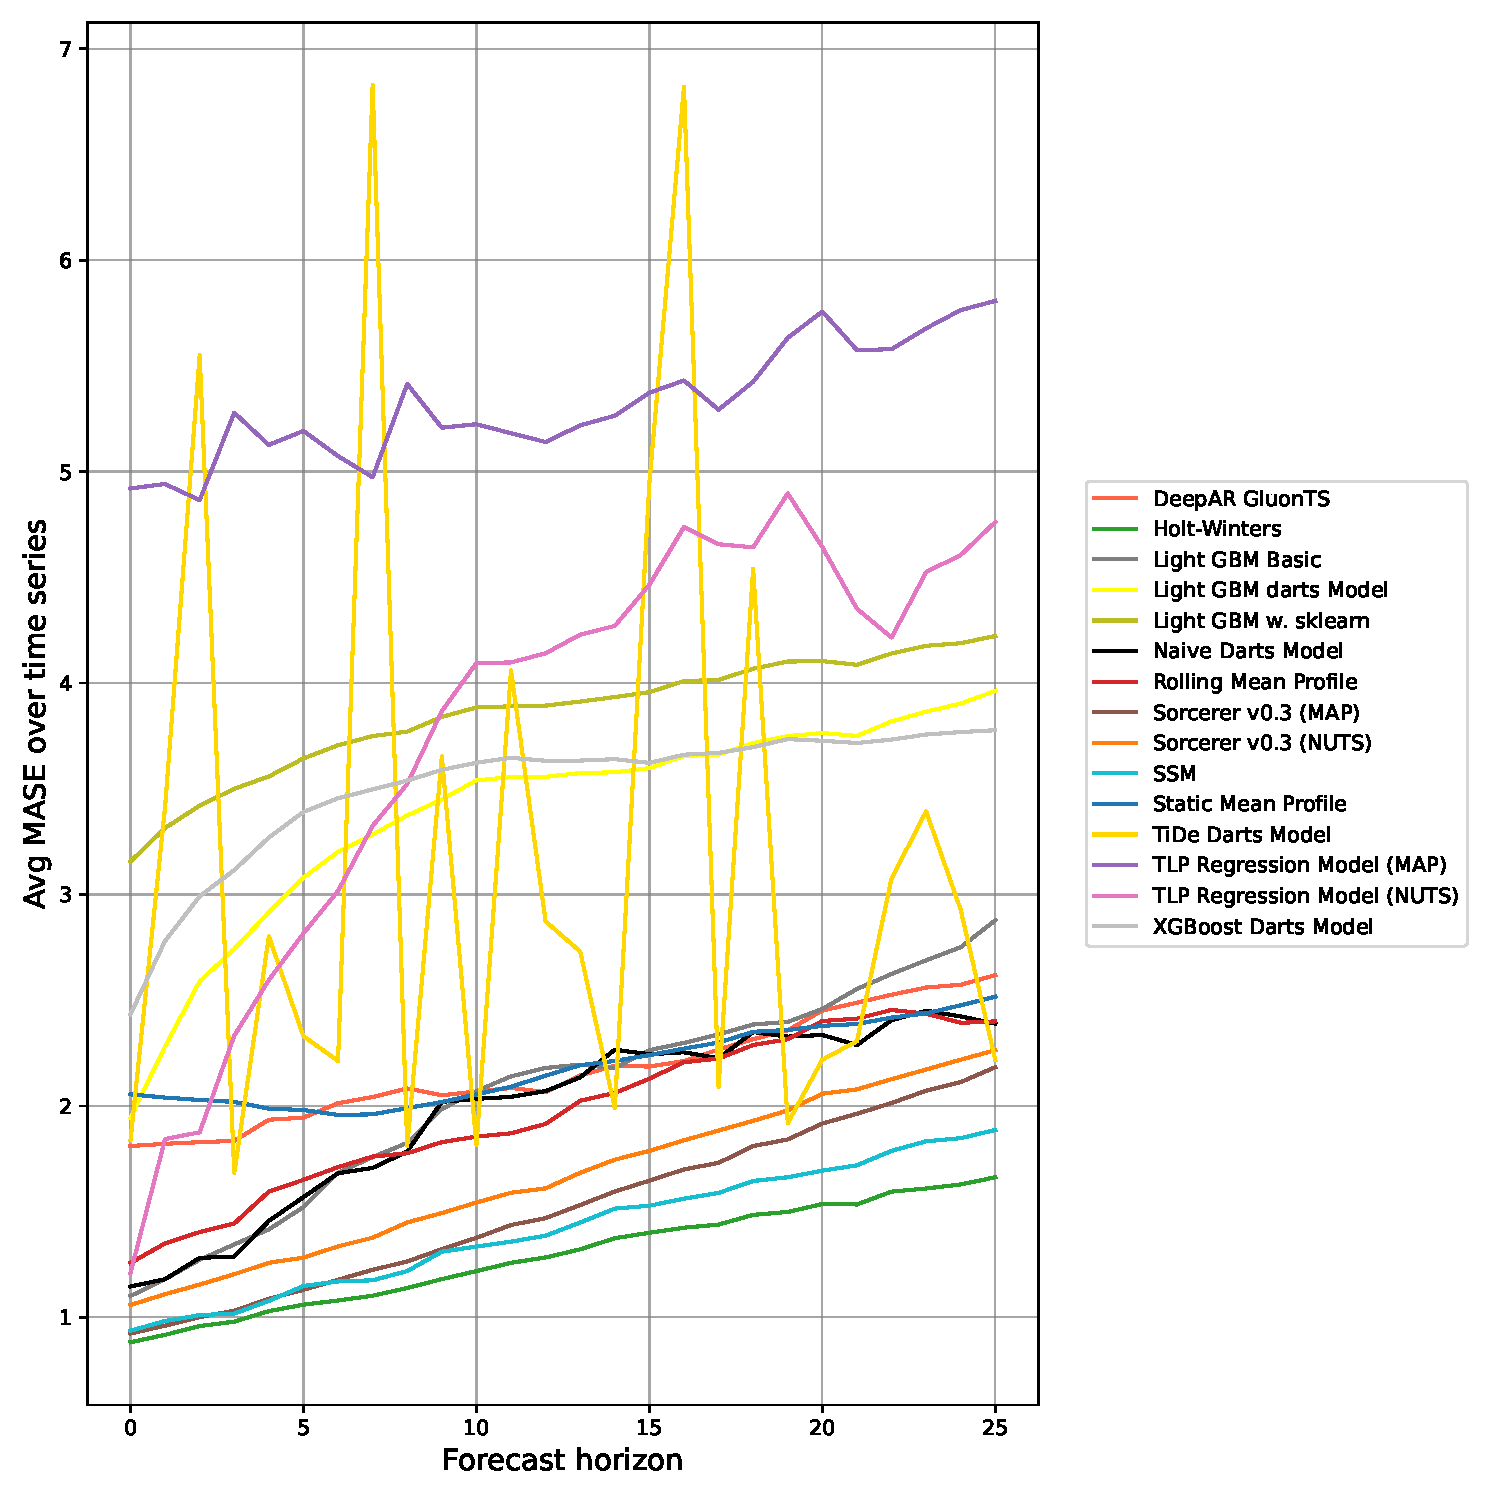
\includegraphics[width=1\textwidth]{./figures/avg_mase_over_time_series.pdf}
	\caption{Average MASE over time series.}
	\label{fig:avg_mase_over_time_series}
\end{figure}

\begin{figure}[h]
	\centering
	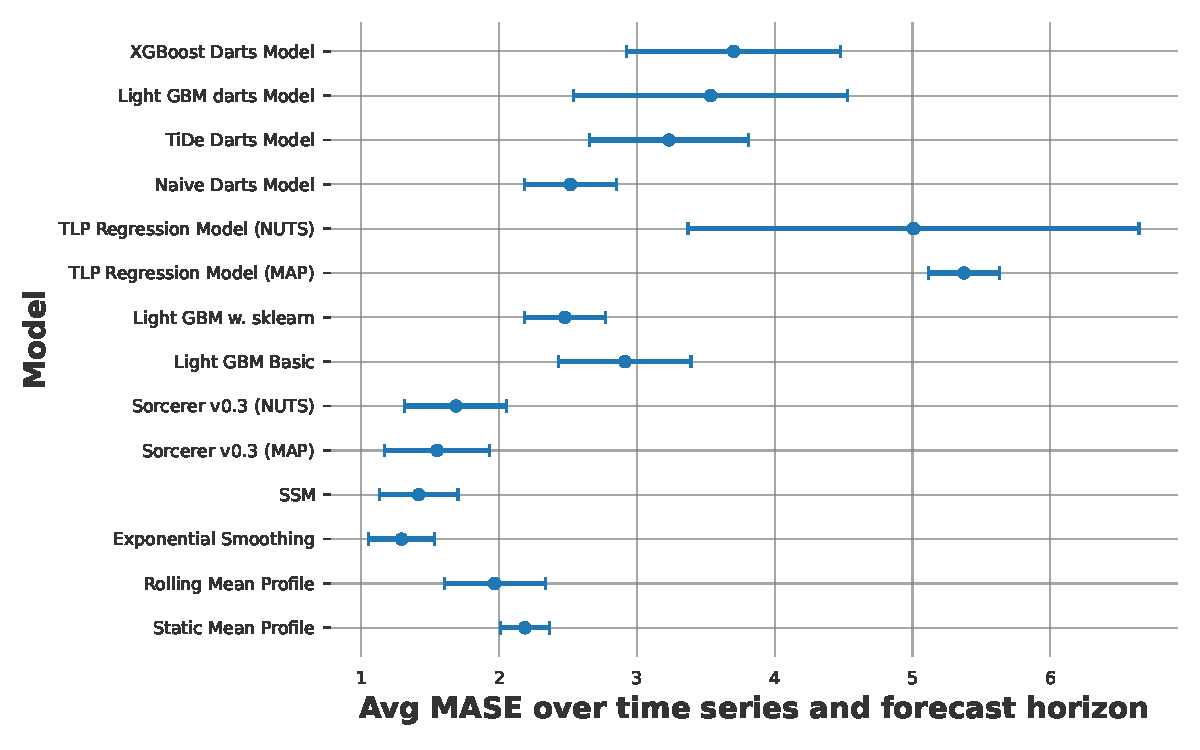
\includegraphics[width=1\textwidth]{./figures/avg_mase_over_time_series_and_forecast_horizon.pdf}
	\caption{Average MASE over time series and forecast horizon.}
	\label{fig:avg_mase_over_time_series_and_forecast_horizon}
\end{figure}


	
%	\newpage
%	\begin{appendices}
%
%	\end{appendices}
	
	
	
	%\bibliographystyle{plainnat}
	%\bibliography{refs}
	
\end{document}